\subsection{Dissecting Inbound Latency}
\label{s:measure_inbound}

%%inbound delay on HP
\begin{figure}
% \subfloat[Flow rate = 100/s, concurrent with \flowmod\ and \packetout\ \label{fig:intel_inbound_test1}]
%   {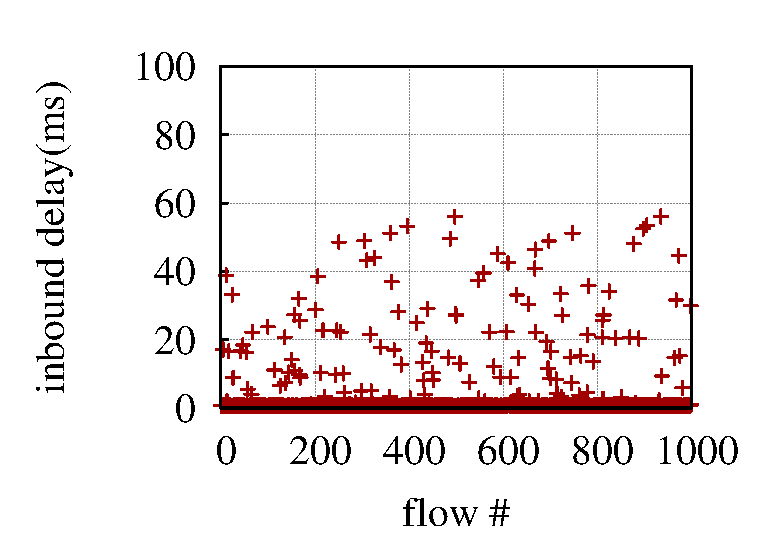
\includegraphics[width=.33\linewidth]{./figs/jan27_intel_inbound_with_pktout_flowmod_rate100.eps}}\hfill
%\subfloat[Flow rate = 200/s\label{fig:hp_inbound_test2}]
%  {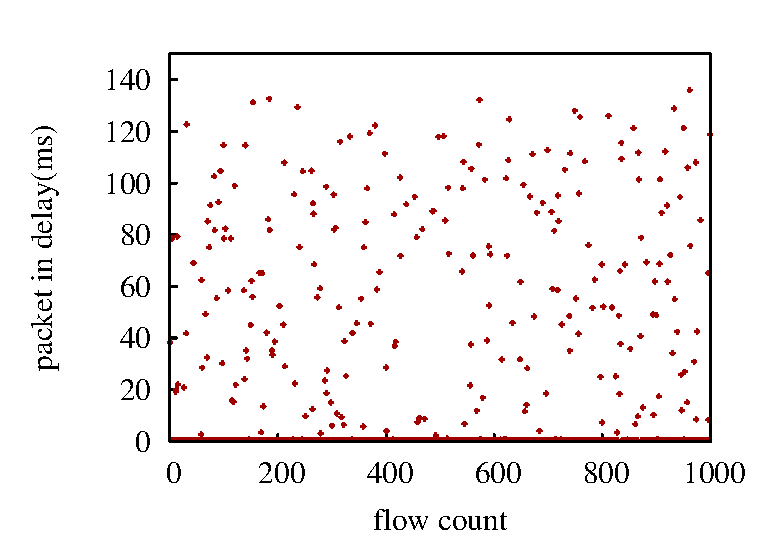
\includegraphics[width=.28\linewidth]{./figs/hp_inbound_delay_200.eps}}\hfill
\subfloat[with flow\_mod/pkt\_out \label{fig:intel_inbound_test3}]
  {\includegraphics[width=.45\linewidth]{./figs/jan27_intel_inbound_with_pktout_flowmod_rate200.eps}}
\subfloat[w/o flow\_mod/pkt\_out \label{fig:intel_inbound_test3_wo}]
  {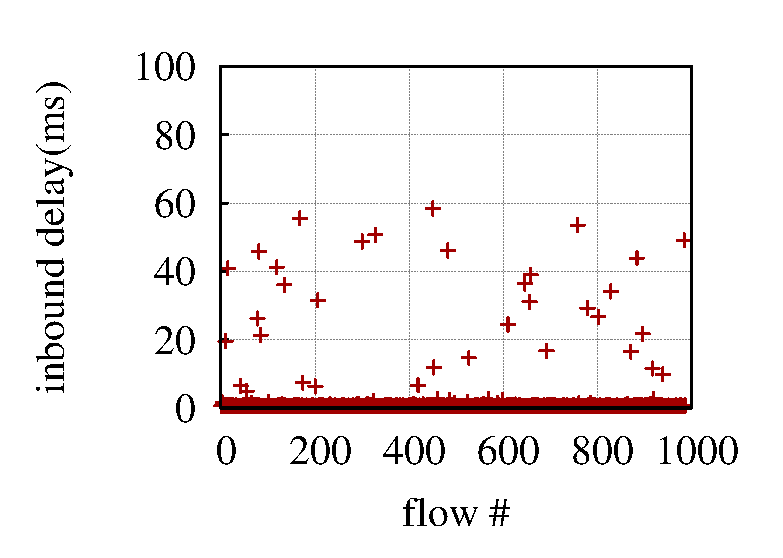
\includegraphics[width=.45\linewidth]{./figs/jan27_intel_inbound_wo_pktout_flowmod.eps}}
\topcompactcaption{{\bf Inbound delay} on {\bf \Intel}, flow arrival rate = 200/s} 
%(a): with concurrent \flowmod\ and \packetout\ operations;
%  (b) without concurrent \flowmod\ and \packetout\ operations}
\label{fig:inbound-1}
\end{figure}

%\emph{Inbound delay:}
To measure inbound latency, we empty the table at the switch, and we generate
traffic such that \packetin events are generated at a certain rate (i.e., we
create packets for new flows at a fixed rate). To isolate the impact of
\packetin processing from other message processing, we perform two kinds of
experiments: (1) the \packetin will trigger corresponding \flowmod (insert
simple OpenFlow rules differing just in destination IP) and \packetout
messages; (2) the\linebreak \packetin message is dropped silently by the
controller. 

We record the timestamp ($t_1$) when each packet is transmitted on the
measurement host's eth1 interface (\figref{experiment_setup}). We also record
the timestamp ($t_2$) when the host receives the corresponding \packetin
message on eth0. The difference ($t_2 - t_1$) is the inbound
latency.\footnote{This measurement technique differs from the approach used
in \cite{ucsdpaper}, where the delay was captured from the switch to the POX
controller which includes the overhead at the controller.}

%\marina{Where are the figures for the inbound delay. Explain how we isolate this
%  type of delay by dropping the pkt at the controller}. 

%%%%HP switch CPU  usage%%%%%%%%%

\begin{table}
\centering
\begin{scriptsize}
\begin{tabular}{cc}
\begin{tabular}{|c|c|c|}
\hline
\multicolumn{3}{|c|}{with flow mod/pkt out} \\ \hline
flow rate & 100/s  & 200/s  \\ \hline
cpu usage & 15.7\%    & 26.5\%   \\ \hline
\end{tabular}
&
\begin{tabular}{|c|c|c|}
\hline
\multicolumn{3}{|c|}{w/o flow mod/pkt out} \\ \hline
flow rate & 100/s   & 200/s \\ \hline
cpu usage & 9.8\%     & 14.4\%   \\ \hline
\end{tabular}
\end{tabular}
\botcompactcaption{CPU usage on \Intel}
\label{fig:inbound-cpu}
\end{scriptsize}
\end{table} 
%\li{is the following sentence correct?}
%When the controller receives \packetin\ message, the controller will drop it. As
%we keep sending packets, it will allow us to repeatedly measure inbound delay. 

Representative results for these two experiments are shown in
\figsref{fig:intel_inbound_test3}{fig:intel_inbound_test3_wo}, respectively,
for the Intel switch; \IBM has similar performance (5ms latency per \packetin on average). 
\BroadcomOne and \BroadcomThree do not support \packetin
messages. For the first experiment, we see that the inbound latency is quite
variable with a mean of 8.33ms, a median of 0.73ms, and a standard deviation
of 31.34ms. For the second experiment, the inbound delay is lower (mean of 
1.72ms, median of 0.67ms) and less variable (standard deviation of 6.09ms). 
We also observe that inbound latency depends on the \packetin rate: e.g. in
first experiment the mean is 3.32 ms for 100 flows/s (not shown) vs. 8.33ms
for 200 flows/s (\figref{fig:intel_inbound_test3}).

The only difference between the two experiments is that in the former case
the switch CPU must process \flowmod and \packetout messages, and send
forwarding entries and outbound packets across the PCIe bus to the ASIC, in
addition to generating \packetin messages. As such, we observe that the CPU
usage is higher when the switch is handling concurrent OpenFlow operations and
generating more \packetin messages (\tabref{fig:inbound-cpu}). However, since
the Intel switch features a powerful CPU (\tabref{switch_para}), plenty of
CPU capacity remains. Our conversations with the switch vendor suggest that
the limited bus bandwidth between the ASIC and switch CPU is the primary
factor contributing to inbound latency. 

%Thus, we conclude
%that the switch CPU is one of the potential causes for the inbound
%latency.\aaron{Do we still think this is true? If the CPU is only 26.5\%
%    utilized, why does latency increase?} Further, our conversations with the
%    switch vendor suggest that the limited bus bandwidth between the ASIC and
%    switch CPU also contributes to the inbound latency. 
%%But they also note that the ASIC-CPU bandwidth is just around 10Mbps.  Thus,
%    %we conclude that inbound delay is mainly caused by switch CPU and due to
%    %interference with \flowmod\ and \packetout\ processing. 
%\sourav {The above lines may have to be re-written. Please check}
 
